\newpage
\subsubsection{QuizziPedia::Back-End::App::Controllers}

\label{QuizziPedia::Back-End::App::Controllers}
\begin{figure}[ht]
	\centering
	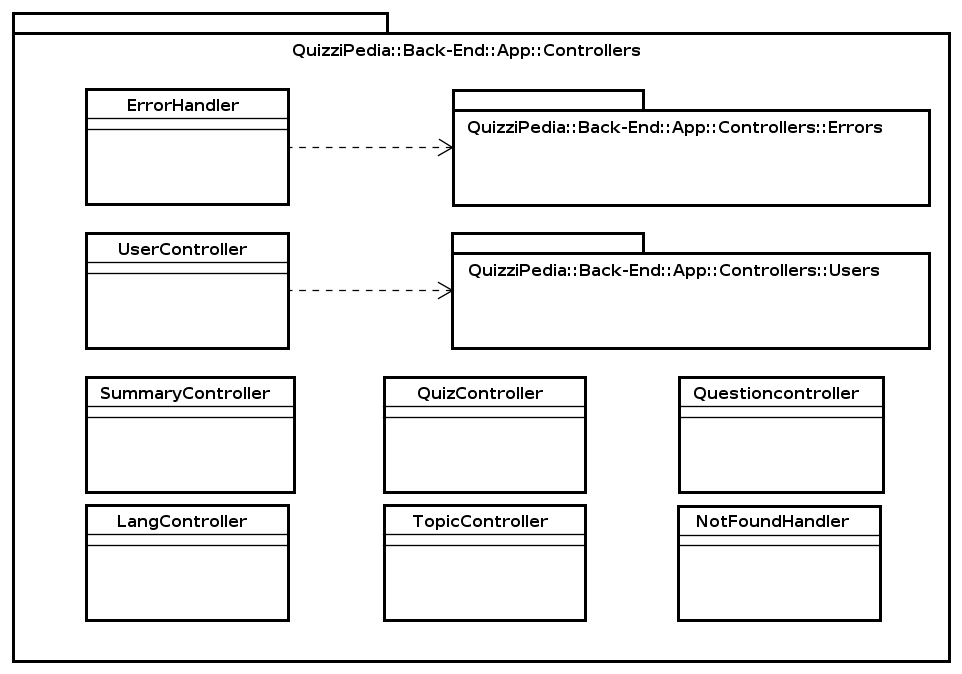
\includegraphics[scale=0.5]{UML/Package/QuizziPedia_Back-End_App_Controllers.png}
	\caption{QuizziPedia::Back-End::App::Controllers}
\end{figure}
\FloatBarrier
	\begin{itemize}
		\item \textbf{Descrizione}:
		\textit{package\ped{G}} contenente i \textit{controllers} di \textit{Express\ped{G}}, definisce la logica dell'applicazione;
		\item \textbf{Padre}: \texttt{App};
		\item \textbf{Interazioni con altri componenti}:
			\begin{itemize}
				\item \texttt{Routers}:
				\textit{package\ped{G}} contenente i router della componente back-end dell'applicazione. Contiene i file di configurazione relativi al routing delle richieste del \textit{client\ped{G}}, ossia i \textit{routers} di \textit{Express\ped{G}};
				\item \texttt{Views}:
				\textit{package\ped{G}} contenente le \textit{\textit{views\ped{G}}} della componente back-end dell'applicazione.
			\end{itemize}
		\item \textbf{Package contenuti}:
			\begin{itemize}
				\item \texttt{Errors}:
				\textit{package\ped{G}} contenente i \textit{controllers\ped{G}} per la gestione degli errori specifici:
					\begin{itemize}
						\item \texttt{QuizziPediaError}: classe che contiene gli errori. Esegue la costruzione del messaggio d'errore specifico per i moduli di \texttt{QuizziPedia::Back-End::App};
					\end{itemize}
				\item \texttt{Users}:
				\textit{package\ped{G}} contenente i \textit{controllers\ped{G}} relativi alla gestione dell'autenticazione e dei dati dell'utente:
				\begin{itemize}
					\item \texttt{AuthentcationController}: classe che si occupa della registrazione e dell'autenticazione dell'utente nel sistema. È un componente ConcreteHandler del design pattern \textit{Chain of responsibility\ped{G}}. Risulta essere il componente che eventualmente esegue la richiesta del client attraverso \textit{Passport\ped{G}};
					\item \texttt{SessionController}: classe \textit{middleware\ped{G}} che, utilizzando \textit{Passport\ped{G}}, si occupa di controllare la consistenza dell'oggetto session durante la sessione associata all'utente autenticato. È un componente ConcreteHandler del design pattern \textit{Chain of responsibility\ped{G}};
					\item \texttt{UserManagementController}: classe che gestisce la logica applicativa riguardante la visualizzazione e la modifica dei dati dell'utente.  È un componente ConcreteHandler del design pattern \textit{Chain of responsibility\ped{G}};
				\end{itemize}
			\end{itemize}
		\item \textbf{Classi contenute}:
		\begin{itemize}
			\item \texttt{ErrorsHandler}: classe \textit{middleware\ped{G}} per la gestione degli errori. Ritorna al client un oggetto di tipo Response con stato HTTP 500 e descrizione dell'errore in formato \textit{JSON\ped{G}}. È un componente ConcreteHandler del design pattern \textit{Chain of responsibility\ped{G}};
			\item \texttt{TopicController}: classe che gestisce la logica applicativa riguardante la visualizzazione e la modifica degli argomenti delle domande;
			\item \texttt{SummaryController}: classe che gestisce la logica applicativa riguardante la visualizzazione e la modifica dei riepiloghi dei questionari;
			\item \texttt{QuizController}: classe che gestisce la logica applicativa riguardante la visualizzazione e la gestione dei questionari;
			\item \texttt{QuestionController}: classe che gestisce la logica applicativa riguardante la visualizzazione, la creazione e la modifica delle domande presenti nell'applicazione;
			\item \texttt{UserController}: classe che raggruppa attraverso require i vari \textit{controllers\ped{G}} responsabili delle operazioni legate alla gestione degli utenti. Si è scelto di predisporre questo raggruppamento per facilitare l'introduzione di nuove funzionalità legate alla gestione degli utenti;
			\item \texttt{LangController}: classe che gestisce la logica applicativa riguardante il passaggio della traduzione delle variabili;
			\item \texttt{NotFoundHandler}: classe che si occupa della gestione dell'errore di pagina non trovata.	Componente ConcreteHandler del design pattern \textit{Chain of responsibility\ped{G}};
		\end{itemize}
	\end{itemize}